\chapter{Componenti di una Data Pipeline}\label{cap:Componenti di una Data Pipeline}
\section{Apache Kafka}
\subsection{Introduzione}
\textbf{Apache Kafka} è una piattaforma \gls{open source}{}, da Jay Kreps, Neha Narkhede e Jun Rao presso LinkedIn e successivamente donata alla \gls{Apache Software Foundation}{} nel 2011. (Figura \ref{fig:logo_kafka}).\\
\textbf{Apache Kafka} nasce con la necessità di LinkedIn di gestire grandi quantità di dati in tempo reale.\\ Già nel 2007 
Jay Kreps e il suo team si resero conto che le soluzioni allora attuali, basate su database tradizionali, non erano in grado di gestire 
un carico di lavoro crescente e la complessità del formato dei dati generati da LinkedIn.\\
Dunque per affrontare tale sfida, nel 2010 LinkedIn iniziò a utilizzare \textbf{Apache Kafka} per gestire i dati di log generati dai vari servizi. \\
Tale adozione ha dimostrato nel tempo che \textbf{Apache Kafka} è in grado di gestire carichi di lavoro molto elevati, di scalare facilmente e di garantire un elevato livello di affidabilità nella consegna di messaggi.\\ 
\textbf{Kafka} è scritto in Java e Scala e rilasciata sotto licenza Apache 2.0. La versione attuale è la 3.5.1 rilasciata il 21 luglio 2023.\\
\textbf{Kafka} nasce originariamente come \gls{message broker} e permette di gestire uno \gls{streaming di eventi}{} in tempo reale. \\ 
In particolare fornisce funzionalità per:
\begin{list}{*}{}
    \item pubblicare e sottoscrivere flussi di eventi, importandoli ed esportandoli da altri sistemi;
    \item archiviare tali flussi in modo affidabile e duraturo;
    \item elabora flussi di eventi in real time o in modo retrospettivo.
\end{list}
\begin{figure}[h]
    \centering
    
\includegraphics[width=0.5\textwidth]{images/componenti/logo_kafka.png}
    \caption{Logo di Apache Kafka}
    \label{fig:logo_kafka}
\end{figure}
\pagebreak
\subsection{Casi d'uso}
\textbf{Apache Kafka} viene ampliamente utilizzato in tutti quelli scenari in cui è richiesto la gestione 
affidabile di grandi quantità di dati in tempo reale.\\
I principali campi di utilizzo di \textbf{Apache Kafka} sono:
\begin{list}{*}
    \item \textbf{messagistica}: \textbf{Apache Kafka} viene particolarmente utilizzato come \gls{message broker}{}, in applicazioni di messaggistica 
    per disaccoppiare la produzione del messaggio dall'elaborazione dello stesso, \textbf{Kafka} rispetto ai tradizionali \gls{message broker}{} offre velocità e \gls{fault tolerance}{};
    \item \item \textbf{elaborazione del flusso dati}: è possibile anche utilizzare \textbf{Kafka} come componente principale per creare \gls{Data Pipeline}{} in cui i dati grezzi,
    provenienti da diverse sorgenti \textbf{Kafka} vengono aggregati, trasformati fino a ottenere un dato elaborato;
    \item \textbf{monitoraggio e analisi}: \textbf{Kafka} può essere utilizzato per raccogliere dati di monitoraggio provenienti da applicazioni, sistemi di controllo o siti web; 
    \item \textbf{archiviazione dei dati}: \textbf{Apache Kafka} può essere utilizzato come sistema di archiviazione dei dati a lungo termine, permettendo così analisi storiche e ripristino di sistemi 
    in caso di guasti;

\end{list}
\subsection{Architettura e funzionamento}
\textbf{Apache Kafka} nasce come sistema distribuito che opera su nodi (Figure \ref{fig:kafka_architecture}), i quali comunicano tramite protocollo o tramite protocollo
\gls{tcp}{} ad alte prestazioni.Data la sua natura distribuita implementa funzionalità di \gls{fault tolerance}{} con possibilità di rimpiazzo dei nodi che hanno avuto un malfunzionamento.\\  
\textbf{Kafka} può essere distribuito e utilizzato in vari modi tra cui \gls{virtual machine}{} e \gls{container}{}, \gls{on-promise}{}, o servizi cloud.\\
In generale \textbf{Apache Kafka} e costituito da due componenti essenziali: server e client.
\subsubsection{server}
\textbf{Kafka} viene eseguito come un cluster di uno o più server, che rivestono diversi ruoli. \\Alcuni svolgono la funzione di \textbf{Kafka Broker}: ricevono i messaggi dai produttori, li archiviano e inviano i messaggi ai rispettivi consumatori, al momento della sottoscrizione.
\\ Altri invece assolvono il compito di \textbf{Kafka Connect}: importano ed esportano i
dati sotto forma di flussi dati, permettendo così  d'interagire con altri sistemi esistenti.
\subsubsection{client}
I \textbf{client} sono un insieme di librerie che consentono di scrivere applicazioni distribuite e microservizi che permettono d'interagire con
il sistema di messaggistica di \textbf{Apache Kafka}, leggendo, scrivendo ed elaborando flussi di messaggi in parallelo, su larga scala e con \gls{fault tolerance}{} anche in caso di
problemi di rete o guasti della macchina.\\
In generale la scelta del client da utilizzare dipende dal linguaggio di programmazione che si vuole utilizzare per sviluppare l'applicazione.
\subsubsection{Produttori e consumatori}
Il produttore \textbf{Kafka} invia i dati, con una richiesta di deposito,  direttamente al \gls{message broker}{}, \textit{Leader} della partizione. Per velocizzare la ricerca del
\textit{Leader}, tutti i nodi possono rispondere alle richieste dei produttori fornendo \gls{metadati}{} su quali nodi sono presenti i \textit{Leader}, tale informazione consentirà al produttore d'indirizzare in modo
appropriato i messaggi.\\
D'altra parte il consumatore emette una richiesta di recupero di messaggi al \gls{message broker}{} che funge da \textit{Leader} della partizione, specificando il suo offset nel registro dei messaggi.\\
Il \gls{message broker}{} risponde con un messaggio contenente il suo offset nel registro con ogni richiesta e con una parte del registro a partire da quella posizione. \\
Per quanto riguarda l'estrazione e il recupero dei messaggi: i dati vengono inviati al broker dal produttore e prelevati dal \gls{message broker}{} dal consumatore. 
\subsubsection{La struttura dei messaggi}
I messaggi inviati all'interno di \textbf{Apache Kafka} sono composti da una chiave, un valore e un timestamp. \\
Oltre a tali informazioni a ogni messaggio viene associato un \gls{topic} o argomento che permette di eseguire operazioni di organizzazione 
e filtraggio dei messaggi.\\
Un messaggio, una volta inviato a un consumatore non viene eliminato dal \gls{topic}{} ma viene mantenuto per un periodo di tempo configurabile attraverso un timeout.\\
I \gls{topic}{} dei rispettivi messaggi vengono partizionati su più nodi per consentire a più consumatori di leggere gli stessi messaggi e permettendo ai client di leggere e scrivere messaggi da/a molti \gls{message broker}{}.\\
Quando un nuovo messaggio viene emesso, quest'ultimo si aggiunge alla rispettiva partizione relativa al \gls{topic}{} e viene assegnato un numero di offset che identifica il messaggio all'interno della partizione.\\
Grazie a tale meccanismo \textbf{Apache Kafka} garantisce che i messaggi vengano letti nell'ordine in cui sono stati scritti.
\subsubsection{Zookeeper}
\textbf{Zookeeper} è un prodotto open-source che si occupa della sincronizzazione tra i cluster distribuiti di sistemi come \textbf{Apache Kafka}. \\
È progettato per gestire operazioni di sincronizzazione, gestione dello stato e configurazioni nei sistemi distribuiti, garantendo coerenza e affidabilità.\\
Il suo funzionamento si basa sul protocollo Zookeeper Atomic Broadcast (ZAB), che è il cuore del servizio di coordinamento di \textbf{Zookeeper}.\\
Ogni nodo invia a intervalli regolari un messaggio \textit{Keep-Alive} a \textbf{Zookeeper}, informandolo così che è vivo e funzionante. Se entro un tempo prestabilito il messaggio non viene ricevuto si presume che il nodo sia
morto e se era un leader se ne elegge un altro.\\
Inoltre \textbf{Zookeeper} permette di definire dei parametri che consentono di capire quando un nodo è guasto e quanto gli altri nodi, appartenenti a una partizione,  sono in ritardo rispetto al \textit{Leader} in termini di sincronizzazione sull'arrivo dei messaggi.\\
Il parametro \textit{zookeeper.session.timeout.ms}, impostato a 6000 millisecondi per impostazione predefinita, indica che, se il leader non riceve l'evento \textit{Keep-Alive} entro quel periodo temporale, detiene che quel nodo sia guasto.\\
Il parametro \textit{replica.lag.max.messages}, indica la massima differenza consentita tra \textbf{Replica's Offset}e \textbf{Leader's Offset}. Se tale differenza è maggiore di \textit{replica.lag.max.message-1}, il nodo viene considerato in ritardo e viene rimosso dall'elenco dei nodi in sincronizzazione dal leader. \\
Tutti i nodi che sono attivi e sincronizzati formano l' \textbf{In-Sync Replica Set}(\textbf{ISR}).\\
Se tutti i nodi in sincronizzazione hanno memorizzato un messaggio nei rispettivi \gls{log}{}, questo messaggio viene considerato confermato e quindi inviato ai consumatori. \\
In questo modo, un sistema come \textbf{Kafka} garantisce che un messaggio di cui è stato eseguito il \textit{commit} non andrà perso, purché sia presente almeno una replica attiva e sincronizzata, in ogni momento.\\
Un nodo non sincronizzato può ricongiungersi all'\textbf{ISR} se può sincronizzarsi completamente di nuovo, anche se ha perso alcuni dati a causa del suo arresto anomalo.
\subsubsection{Politiche di retentions}
Con \textbf{Retention} in \textbf{Kafka} si intende la possibilità di controllare la dimensione dei registri
degli argomenti ed evitare di superare le dimensioni del disco esistente.\\
La conservazione può essere configurata o controllata in base alla dimensione dei \gls{log}{} o in
base alla durata configurata. Tale configurazione può essere impostata a grana fine o a
grana grossa per ogni argomento o per tutti gli argomenti.
\paragraph{Retention basata sulle dimensione}
Una volta raggiunto il tempo di conservazione configurato per il segmento, quest'ultimo viene contrassegnato per l'eliminazione o la \gls{compattazione}{} in base al criterio di pulizia configurato. Il periodo di conservazione predefinito per i segmenti è di 7 giorni.
I parametri configurabili per la \textbf{Retention} basata sul tempo sono in ordine d'importanza e valutazione sono:
\begin{enumerate}
    \item $log.retention.ms$;
    \item $log.retention.minutes$;
    \item $log.retention.hours$.
\end{enumerate}
Nel momento in cui un parametro di livello di priorità superiore non è impostato si segue la politica di conservazione del parametro di livello di priorità inferiore.\\
\paragraph{Retention basata sulla dimensione}
In questo caso si va configurare la dimensione massima di una struttura di dati di registro per una partizione di argomento. Una volta che la dimensione del registro raggiunge questa dimensione, inizia a rimuovere i segmenti dalla sua fine.\\
\pagebreak
\\
I parametri configurabili per la \textbf{Retention} basata dimensione sono in ordine d'importanza e valutazione:
\begin{enumerate}
    \item $log.segment.bytes$: la dimensione massima di un singolo file di registro;
    \item $log.retention.check.interval.ms$: la frequenza in millisecondi con cui la pulizia del registro verifica se un registro è idoneo per l'eliminazione;
    \item $log.segment.delete.delay.ms$: la quantità di tempo da attendere prima di eliminare un file dal file system.
\end{enumerate}

\subsubsection{I replicas}

\begin{figure}[h]
    \centering
    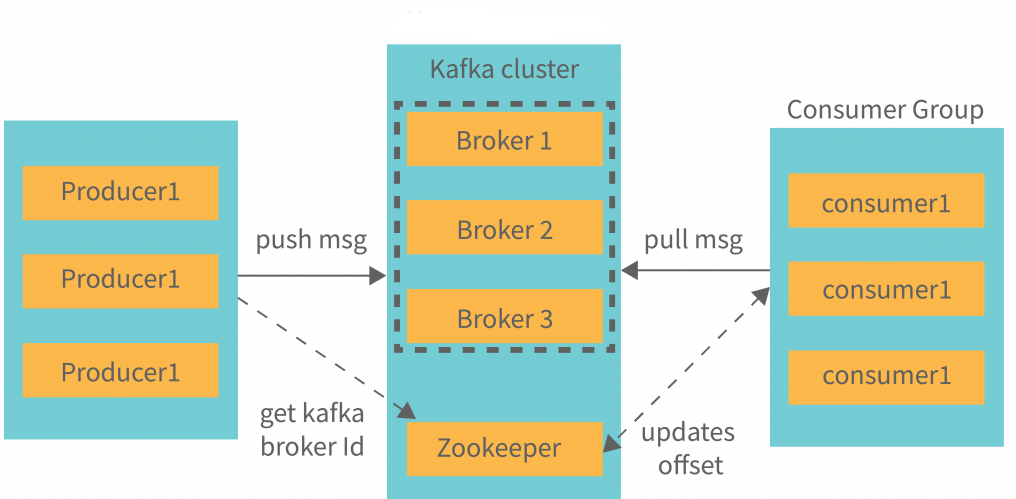
\includegraphics[width=0.9\textwidth]{images/componenti/kafka_architetcture.png}
    \caption{Architettura di Apache Kafka}
    \label{fig:kafka_architecture}
\end{figure}

\subsection{Garanzie di funzionamento}
In \textbf{Kafka} esistono produttori e consumatori che producono e sottoscrivono eventi. Gli uni, essendo in un ambiente distribuito,
sono indipendenti l’uno dall’altro. \\
\textbf{Apache Kafka} in tale contesto può fornire una delle seguenti garanzie sulla consegna e ricezione dei messaggi:
\begin{list}{*}
    \item \textbf{at most once}: i messaggi vengono consegnati al consumatore al più una volta. In questo caso, i messaggi possono essere persi, ma non duplicati;
   \item \item  \textbf{at least once}: i messaggi vengono consegnati al consumatore almeno una volta, i messaggi possono essere duplicati, ma non persi;
    \item \textbf{exactly once}: i messaggi vengono consegnati al consumatore esattamente una volta. In questo caso, i messaggi non vengono né persi né duplicati, è la garanzia più costosa ma maggiormente richiesta.
\end{list}

\subsection{Il pattern Publisher-Subscriber}

\pagebreak
\section{Apache Druid}

\begin{figure}[h]
    \centering
    
\includegraphics[width=0.5\textwidth]{images/componenti/logo_druid.png}
    \caption{Logo di Apache Druid}
    \label{fig:logo_druid}
\end{figure}
\section{Streaming Data Pipelines}
\newpage
\pagestyle{empty}
\null % o \mbox{} o \phantom{X}
\newpage